% id: 113-01
% book: 베이직쎈 확률과 통계 · 06 이항분포와 정규분포
% section: 유형 066 정규분포곡선의 성질
% figure: tikz:fig-113-01
% answer: 
% answer_source: 
% variant_level: 0 (원본 전사)
% 이 파일은 build.mjs 가 items.json 에서 만든다. 고칠 때는 items.json 을 고친다.
\smash{\raisebox{1.5mm}{\dmkichul{베이직쎈 확률과 통계 113쪽 01번}}}
\noindent\begin{minipage}[t]{0.58\linewidth}\vspace{0pt}\raggedright 오른쪽 그림의 두 곡선 $\mathrm{A}$, $\mathrm{B}$는 각각 정규분포 $\mathrm{N}(m_{\mathrm{A}}{,}\mkern3mu\mathopen{}{\sigma_{\mathrm{A}}}^2)$, $\mathrm{N}(m_{\mathrm{B}}{,}\mkern3mu\mathopen{}{\sigma_{\mathrm{B}}}^2)$을 따르는 두 확률변수의 정규분포곡선이다. $m_{\mathrm{A}}$와 $m_{\mathrm{B}}$, $\sigma_{\mathrm{A}}$와 $\sigma_{\mathrm{B}}$의 대소 관계로 옳은 것은?\end{minipage}\hfill\begin{minipage}[t]{0.4\linewidth}\vspace{0pt}\centering \resizebox{\ifdim\width>\linewidth\linewidth\else\width\fi}{!}{% 113-01(인쇄 113쪽) — 유형 066 01번의 두 정규분포곡선 A, B(대칭축은 같고 A 가 높고 좁으며 B 가 낮고 넓다 · 대칭축은 점선).
% 스캔 화질이 낮아 TikZ 로 다시 그림. 라벨은 원문에 있는 것만(A, B, x)이고 평균·표준편차의 값은 적지 않는다.
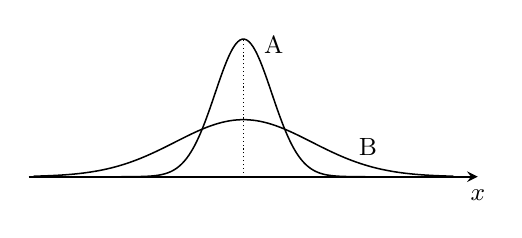
\begin{tikzpicture}[x=0.62cm, y=1.15cm, line width=0.55pt, font=\small]
  \draw[->, >=stealth, line width=0.7pt] (-4.4,0) -- (4.8,0) node[below=1pt] {$x$};
  \draw plot[domain=-2.5:2.5, samples=110, smooth] ({\x},{1.52*exp(-\x*\x/(2*0.58*0.58))});
  \draw plot[domain=-4.3:4.3, samples=110, smooth] ({\x},{0.63*exp(-\x*\x/(2*1.40*1.40))});
  \draw[densely dotted, line width=0.4pt] (0,0) -- (0,1.52);
  \node at (0.62,1.45) {$\mathrm{A}$};
  \node at (2.55,0.33) {$\mathrm{B}$};
\end{tikzpicture}
}\end{minipage}\par
\begin{choicesii}{$m_{\mathrm{A}}=m_{\mathrm{B}}$, $\sigma_{\mathrm{A}}>\sigma_{\mathrm{B}}$}{$m_{\mathrm{A}}=m_{\mathrm{B}}$, $\sigma_{\mathrm{A}}<\sigma_{\mathrm{B}}$}{$m_{\mathrm{A}}>m_{\mathrm{B}}$, $\sigma_{\mathrm{A}}>\sigma_{\mathrm{B}}$}{$m_{\mathrm{A}}>m_{\mathrm{B}}$, $\sigma_{\mathrm{A}}<\sigma_{\mathrm{B}}$}{$m_{\mathrm{A}}<m_{\mathrm{B}}$, $\sigma_{\mathrm{A}}=\sigma_{\mathrm{B}}$}\end{choicesii}
